\documentclass{article}\usepackage[]{graphicx}\usepackage[]{color}
% maxwidth is the original width if it is less than linewidth
% otherwise use linewidth (to make sure the graphics do not exceed the margin)
\makeatletter
\def\maxwidth{ %
  \ifdim\Gin@nat@width>\linewidth
    \linewidth
  \else
    \Gin@nat@width
  \fi
}
\makeatother

\definecolor{fgcolor}{rgb}{0.345, 0.345, 0.345}
\newcommand{\hlnum}[1]{\textcolor[rgb]{0.686,0.059,0.569}{#1}}%
\newcommand{\hlstr}[1]{\textcolor[rgb]{0.192,0.494,0.8}{#1}}%
\newcommand{\hlcom}[1]{\textcolor[rgb]{0.678,0.584,0.686}{\textit{#1}}}%
\newcommand{\hlopt}[1]{\textcolor[rgb]{0,0,0}{#1}}%
\newcommand{\hlstd}[1]{\textcolor[rgb]{0.345,0.345,0.345}{#1}}%
\newcommand{\hlkwa}[1]{\textcolor[rgb]{0.161,0.373,0.58}{\textbf{#1}}}%
\newcommand{\hlkwb}[1]{\textcolor[rgb]{0.69,0.353,0.396}{#1}}%
\newcommand{\hlkwc}[1]{\textcolor[rgb]{0.333,0.667,0.333}{#1}}%
\newcommand{\hlkwd}[1]{\textcolor[rgb]{0.737,0.353,0.396}{\textbf{#1}}}%
\let\hlipl\hlkwb

\usepackage{framed}
\makeatletter
\newenvironment{kframe}{%
 \def\at@end@of@kframe{}%
 \ifinner\ifhmode%
  \def\at@end@of@kframe{\end{minipage}}%
  \begin{minipage}{\columnwidth}%
 \fi\fi%
 \def\FrameCommand##1{\hskip\@totalleftmargin \hskip-\fboxsep
 \colorbox{shadecolor}{##1}\hskip-\fboxsep
     % There is no \\@totalrightmargin, so:
     \hskip-\linewidth \hskip-\@totalleftmargin \hskip\columnwidth}%
 \MakeFramed {\advance\hsize-\width
   \@totalleftmargin\z@ \linewidth\hsize
   \@setminipage}}%
 {\par\unskip\endMakeFramed%
 \at@end@of@kframe}
\makeatother

\definecolor{shadecolor}{rgb}{.97, .97, .97}
\definecolor{messagecolor}{rgb}{0, 0, 0}
\definecolor{warningcolor}{rgb}{1, 0, 1}
\definecolor{errorcolor}{rgb}{1, 0, 0}
\newenvironment{knitrout}{}{} % an empty environment to be redefined in TeX

\usepackage{alltt}

\usepackage{graphicx} 
\usepackage{geometry} 
\geometry{left=1in, right=1in, top=1in, bottom=1in}
\usepackage{hyperref}
\usepackage{parskip}
\linespread{1.2}
\IfFileExists{upquote.sty}{\usepackage{upquote}}{}
\begin{document} % -------------------------------------------------------------

\begin{center}
\Large \bfseries R Requirements for MFE Students
\end{center}

\bigskip

\subsection*{Intro} % ----------

This document will walk you through various pieces of software that you need to download in order to get up and running with R. These include the R language itself, as well as a friendly environment (RStudio) in which to write your R code (this is called an ``integrated developement environemt'' or IDE for short). In addition, we ask that you have a Latex installation on your computer (for writing fancy math) and that your R environment is capable of producing RMarkdown documents, which is a type of document that let's you put normal text, math formulas, R code, and R output together very easily. These RMarkdown documents are a great way to do your homework; they're like Jupyter notebooks except that they easily compile (ie, convert) to well-formatted PDF documents.

\subsection*{R} % ----------

R is software for data analysis. It's like Python, but geared toward statistical work; it's like Stata, but better for programming; it's like Matlab, but free.
 
You need to download and install R onto your computer. R is hosted on the ``Comprehensive R Archive Network'' (aka CRAN). It's not the prettiest website out there. To download R, go to \url{https://cran.r-project.org/} (the top link if you Google ``R Cran'') and click on the download link for your operating system (Linux, Mac OSX, or Windows). Depending on your OS, you'll be taken to a second page where you have to choose which ``version'' or ``package'' to download. Linux users should choose their flavor of Linux (Debian, Ubuntu, etc.); Mac users should pick the top link (R-4.1.1.pkg); Windows users should choose ``Base'' and then click the download link at the top of the next page. After R downloads, install it as you would any other piece of software.

For Python users that have downloaded the Anaconda suite of software: R is included in that bundle. You are welcome to use that version of R. However, the R program via Anaconda is stored in a different directory than the default location used when you install R via CRAN. If you encounter any errors using R via Anaconda, the usual fix involves changing the path to the directory where R is located.

\begin{center}
  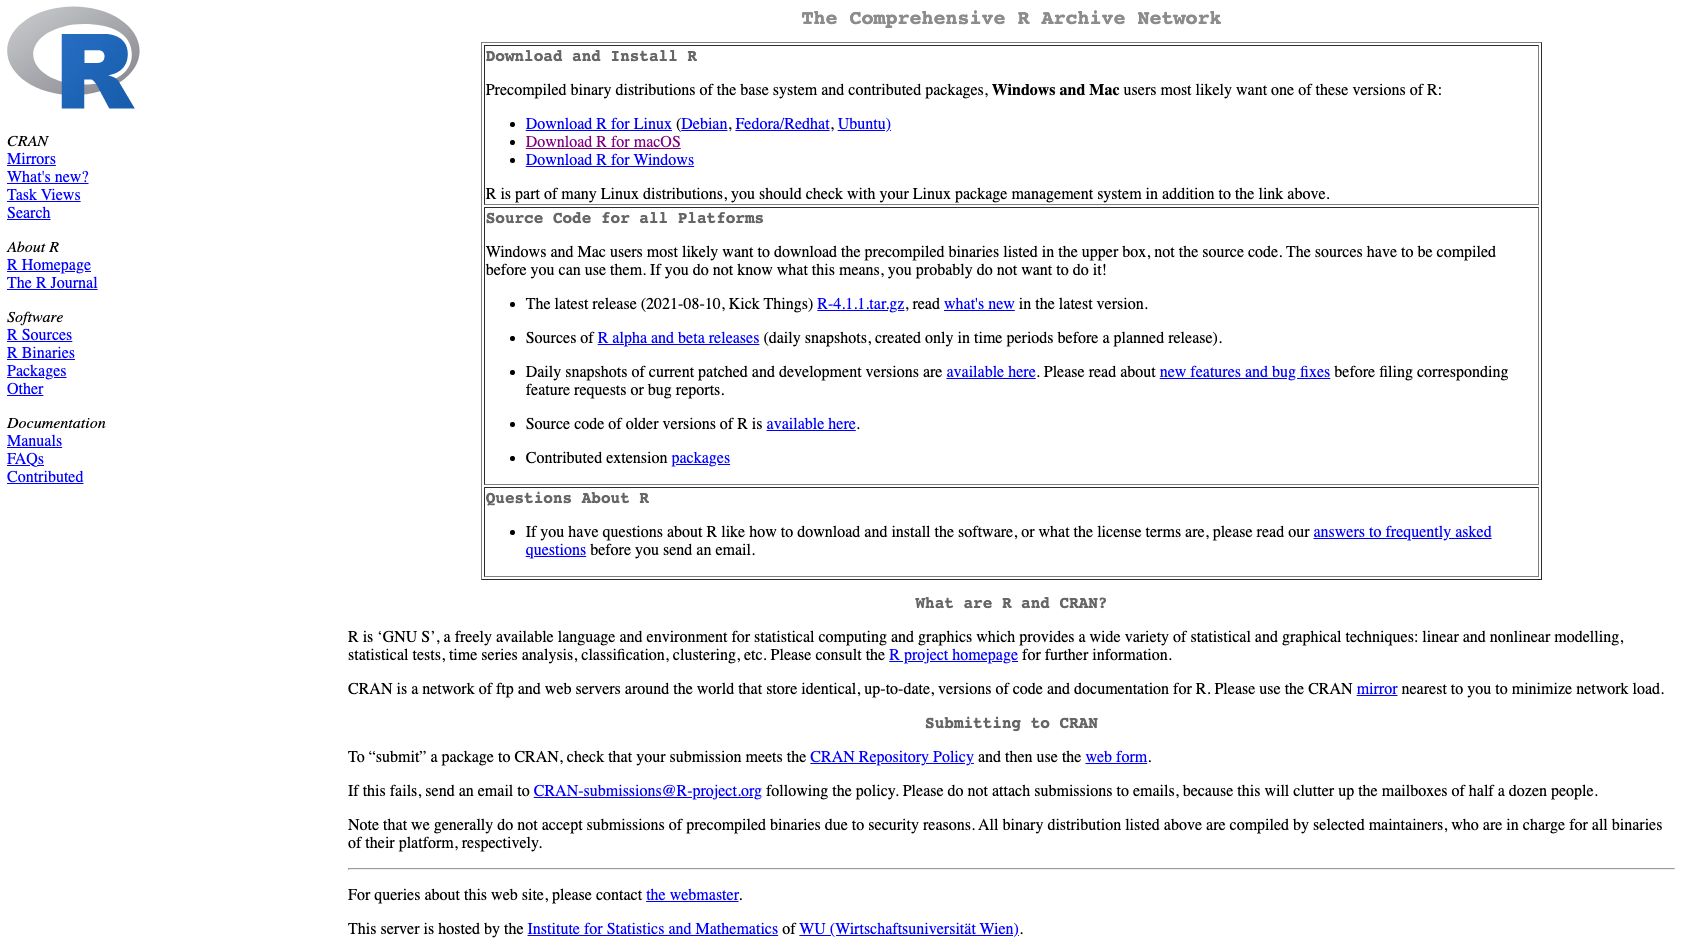
\includegraphics[width=0.8\linewidth,keepaspectratio]{cran.png}
\end{center}

Once you've installed R, open up the application. It will be basic. You'll get one floating window called the ``R Console'' or ``R Terminal'' with a bunch of text and a command prompt.

\begin{center}
  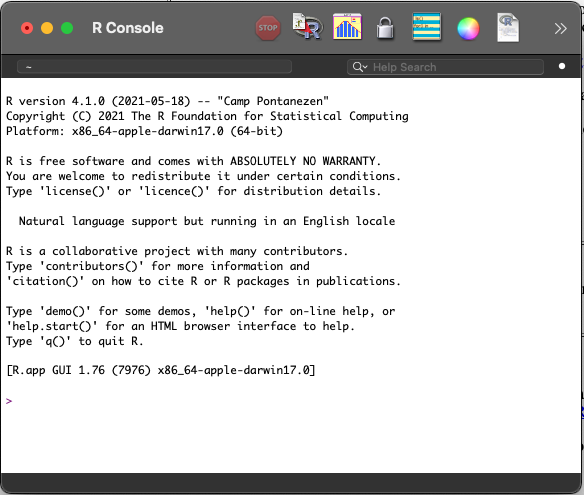
\includegraphics[width=0.5\linewidth,keepaspectratio]{r_console.png}
\end{center}

At the prompt (which looks like a greater-than sign, $>$) type \texttt{2+2} and hit enter. This text (2+2) will be parsed and evaluated by R, and the value of the expression (4) will be returned:

\begin{knitrout}
\definecolor{shadecolor}{rgb}{0.969, 0.969, 0.969}\color{fgcolor}\begin{kframe}
\begin{alltt}
\hlnum{2}\hlopt{+}\hlnum{2}
\end{alltt}
\begin{verbatim}
## [1] 4
\end{verbatim}
\end{kframe}
\end{knitrout}

We'll cover why there's a \texttt{[1]} to start the line on the first day of our workshop.

Using R via this simple application window and a command prompt works just fine, but it's a pretty unfriendly way to use R, so close the R application. To make the experience with R friendlier, you'll want an IDE. My favorite IDE for R is RStudio. You're welcome to use any IDE that you like, but this document will be specific to RStudio. (You'll have to figure out the rest of this on your own if you go with another editor or IDE like Atom, Jupyter, Sublime, or VS Code.)

\subsection*{RStudio} % ----------

You need to download and install RStudio. To do so, go to \url{https://www.rstudio.com/}. At the top, click on ``Products'' and then ``RStudio''. Choose ``Desktop'' and then ``Download RStudio Desktop''. Once downloaded, install it.

Open up RStudio. It should find the R application you previously installed (if not, this is usually where Jupyter users need to ``point'' RStudio to R. See this \href{https://support.rstudio.com/hc/en-us/articles/200486138-Changing-R-versions-for-RStudio-desktop}{link} for more info.) 

\begin{center}
  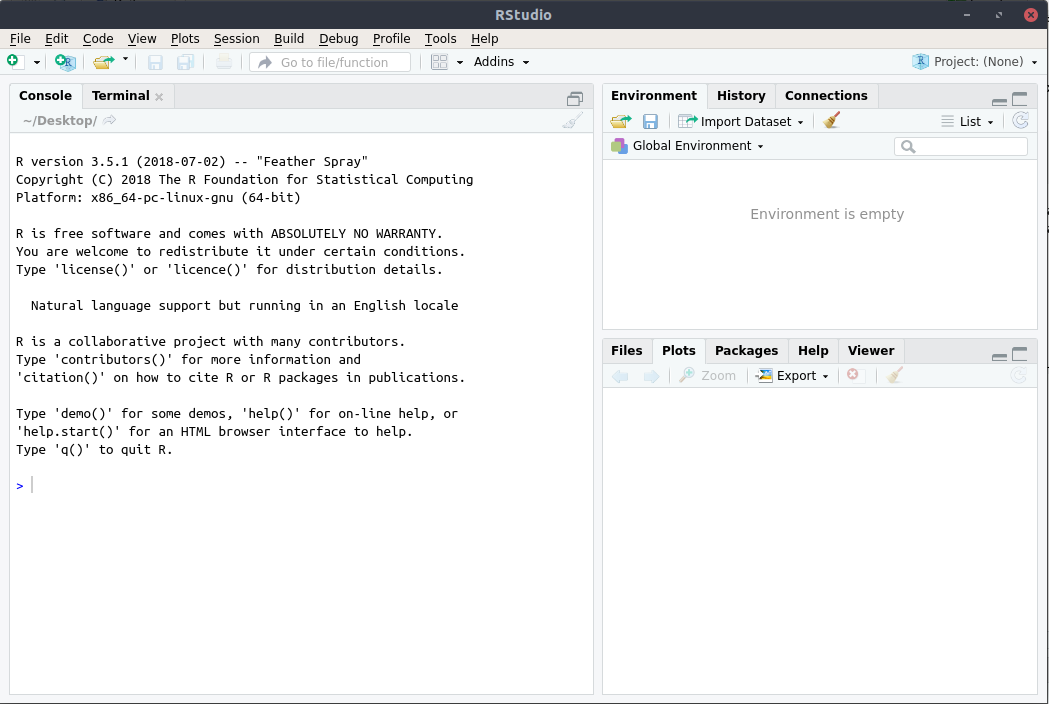
\includegraphics[width=0.5\linewidth,keepaspectratio]{rstudio_screenshot.png}
\end{center}

On the bottom left side of the screen in a window called ``Console'', again type \texttt{2+2} and hit enter. R will return \texttt{4}. 

Next, type:

\begin{knitrout}
\definecolor{shadecolor}{rgb}{0.969, 0.969, 0.969}\color{fgcolor}\begin{kframe}
\begin{alltt}
\hlstd{x} \hlkwb{=} \hlnum{3}\hlopt{+}\hlnum{7}
\end{alltt}
\end{kframe}
\end{knitrout}

Now you'll see the object \texttt{x} in the ``Environment'' window on the top right. Go back to the console on the left and type \texttt{x} and hit return. R will return \texttt{10}. Yay - things are working!

\subsection*{RMarkdown} % ----------

Let's say we don't want to just write R code, but we want the code, some results or graphics from our code, and some floating text (like paragraphs explaining what the code does) all to show up in the same document. R and RStudio provide a way to make that kind of document. In fact, there are two related options. The first is an RMarkdown document that can be easily converted to PDF (and turned in as a homework assignment). The second is an R Notebook and, much like a Jupyter Notebook, the results of your code live in-line in the document alongside your code. For now, we're going to focus on first option.

Unlike what-you-see-is-what-you-get text editing programs like Microsoft Word, with an RMarkdown document you ``code'' your document, including the document's contents \emph{and} its formatting. That means, for example, that you write ``\textbackslash beta'' and when you compile the document, you see ``$\beta$''. Or, as another example, you code \_word\_ in order to set ``word'' in italics, like so: \emph{word}. For a little intro on the RMarkdown language, check out this site: \url{https://rmarkdown.rstudio.com/lesson-1.html}.

Let's create our first RMarkdown document. In RStudio, click on the dropdown arrow next to the icon for a new document (this is at the top left of RStudio), then choose ``RMarkdown''. The first time you do this RStudio may tell you that it needs to install packages, say yes/ok and let those install. If there is any error with this step, go to the bottom right window in RStudio and click on the tab called ``Package''. Then click ``Install''. Type ``rmarkdown'' (all lowercase and without the quotes) and click ``Install''. Once you've got the packages installed, go back to the blank page icon at the top left and create a new RMarkdown document. 

A diaglog box will pop up asking for you to provide a document title and author, it also gives you the option to select ``html'' or ``pdf'', among other things. 

\begin{center}
  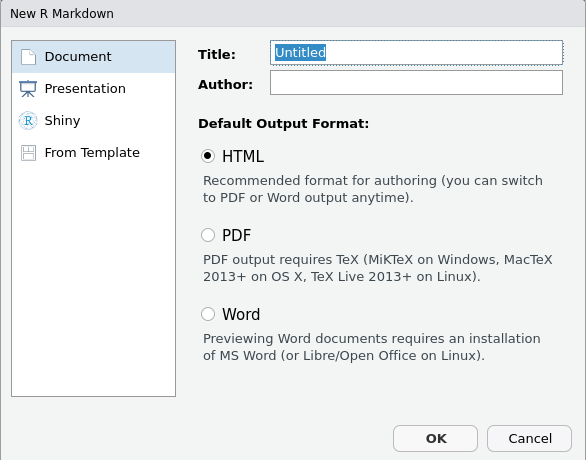
\includegraphics[width=0.5\linewidth,keepaspectratio]{rmarkdown_popup.png}
\end{center}

Right now, you have enough software to make an html document, but you don't have enough to create a pdf. For that, you need Latex. Hit ``Cancel'' and quit RStudio; let's go get Latex.

\subsection*{Latex} % ----------

TeX (with the ``La'' in front and from now on I won't capitalize the X) is a computer program for typesetting documents. This means you enter text into any basic text editor, and Tex will compile those your text and instructions into a document. This provides the user the ability to create many symbols (like $\bar{x} = \sum_{i=1}^n x_i$) and provide precise formatting to a document. Although Tex is a super-stable piece of software created by Donald Knuth, it is incredibly unfriendly to use. But, Tex is like Microsoft Word for people who write math -- everybody in academia uses Tex -- so we need to learn how to use it as well. Thankfully a computer scientist named Leslie Lamport made LaTeX (pronounced la-tech, and henceforce written Latex). Latex is a set of macros for TeX that takes the experience of working with Tex from horrible to somewhat-manageable. (In my experience, there is no good/fun way to write Tex/Latex, so ``somewhat-manageable'' is the best we can do.) 

You need to install Latex and doing so will automatically install Tex for you. Latex has a bunch of different ``flavors'' (the more correct word is ``distributions'') named MacTex (for Mac folks) or MikTex (for Windows) and a few others -- for our purposes they're all basically the same. Go to \url{https://www.Latex-project.org/get/} and use the links to find and download Latex for your OS (Linux users should already have Latex installed). You are welcome to install a ``full'' Latex distribution (usually  about 3GB in size) or a smaller Latex distribution that contains just a core set of functionality (called BasicTex or something similar). If you install MikTex on Windows, it automatically installs just the core functionality and then auto-downloads additional packages as you need them. However, it does this in a annoying way where by default you are prompted every time MikTex needs to download a Tex package. You don't want this and it will cause problems when compiling RMarkdown documents. To change the MikTex default, go to the MikTex Console App, click ``Settings'' and then change the missing package setting from ``ask me'' to ``always install missing packages on the fly.''

We'll be using Tex/Latex as an intermediate step when creating pdf documents. In fact, if we do everything right, you may not even notice that Tex is being used. However, if you want to write Latex documents (without R or RMarkdown, just pure Latex) and compile them straight to pdf, you can download an editor for Latex (this is like how we will use RStudio for R). I use TexMaker, but there are lots of options including add-ons in VS Code, and you should feel free to get whichever you like (or none of them -- since we'll mostly be using Latex via RStudio).

\subsection*{Getting It All Working} % ----------

Let's see if we can get everything working. On your computer, create a new directory (also known as a folder). Open RStudio (if you closed it earlier). Create a new RMarkdown document (either by going to File $>$ New File $>$ RMarkdown or by doing the same via the little white icon with the green plus in the top left corner of RStudio). Choose PDF and hit OK. The new document is pre-populated with some template text, just leave that there. Save this document in the directory you just created.

Before we compile this document from the raw text you see in RStudio to a nice little PDF, we need to change one setting. Go to RStudio's ``Tools'' menu and click ``Global Options''. Click ``Sweave'' on the left and then change the top dropdown from ``Sweave'' to ``Knitr''. Then exit global options.

Back in your new RMarkdown document, click the ``Compile PDF'' button toward the top-left of the screen (you can also go to File $>$ Compile PDF or use the shortcut Ctrl+Shift+K). A new tab will open near the ``Console'' in the bottom-left called ``RMarkdown''. If everything works, in a couple seconds, a PDF will pop up. If not, there will be an error message in the ``RMarkdown'' tab. If you get an error, Google that error and try to fix your problem. If you can't resolve it on your own, email me.

If you are able to create the PDF document then you're all set up. See you soon.

\bigskip

\textbf{-Dan Yavorsky}

Email: dyavorsky@gmail.com 

Cell: 951-201-0927

LinkedIn: \url{https://www.linkedin.com/in/dyavorsky/}

\end{document}
